% =====================================================================
%  SLIDE TRÌNH BÀY — Payment Intelligence Ecosystem
%  Template: Beamer + theme Metropolis (Matthias Vogelgesang, CC-BY-SA 4.0).
%  Biên dịch: make slides   (hoặc: xelatex slides.tex, chạy 2 lần)
%  Biểu đồ: figures/*.pdf, sinh bằng make slides-figures từ results/ và lần chạy tuning.
%  Số test và số bộ report chỉ TRÍCH LẠI từ results/published.json (test-một-lần).
% =====================================================================
\documentclass[aspectratio=169,11pt]{beamer}
\usetheme[progressbar=frametitle,numbering=fraction,block=fill]{metropolis}

\usepackage{fontspec}
\setsansfont{TeX Gyre Heros}
\setmonofont{DejaVu Sans Mono}[Scale=0.82]
\usepackage[vietnamese]{babel}
\usepackage{booktabs,array,tabularx}
\usepackage{tikz}
\usetikzlibrary{arrows.meta,positioning,shapes.geometric,calc,fit,backgrounds,shadows}
\usepackage{fontawesome5}

% ---------- Màu ----------
\definecolor{navy}{HTML}{1B2A4A}
\definecolor{s1}{HTML}{2A78D6}
\definecolor{s2}{HTML}{EB6834}
\definecolor{s3}{HTML}{1BAF7A}
\definecolor{muted}{HTML}{C3C2B7}
\definecolor{ink2}{HTML}{52514E}
\definecolor{soft}{HTML}{EEF4FC}
\definecolor{good}{HTML}{0CA30C}
\definecolor{bad}{HTML}{D03B3B}
\definecolor{page}{HTML}{FAFAF8}
\setbeamercolor{frametitle}{bg=navy,fg=white}
\setbeamercolor{progress bar}{fg=s1,bg=muted!40}
\setbeamercolor{title separator}{fg=s1}
\setbeamercolor{background canvas}{bg=page}
\setbeamercolor{alerted text}{fg=s2}
\setbeamercolor{block title}{bg=soft,fg=navy}
\setbeamercolor{block body}{bg=soft!50}
\setbeamercolor{block title alerted}{bg=s2!15,fg=s2!80!black}
\setbeamercolor{block body alerted}{bg=s2!6}
\setbeamercolor{block title example}{bg=good!15,fg=good!60!black}
\setbeamercolor{block body example}{bg=good!5}

\newcommand{\num}[1]{\textbf{\color{navy}#1}}
\newcommand{\quoted}{\,{\scriptsize\color{ink2}(trích lại)}}
\newcommand{\src}[1]{{\scriptsize\color{ink2}\texttt{#1}}}

\tikzset{
  box/.style={rounded corners=3pt,draw=#1,fill=#1!8,line width=0.8pt,align=center,
    font=\footnotesize,inner sep=4pt},
  box/.default=s1,
  pstep/.style={rounded corners=3pt,draw=navy!60,fill=white,align=center,font=\scriptsize,
    minimum height=9mm,text width=17mm,inner sep=2pt},
  arr/.style={-{Stealth[length=2mm]},line width=0.8pt,color=ink2},
  c/.style={box=#1,text width=31mm,minimum height=10mm,font=\scriptsize},
  c/.default=s1,
}

\title{Payment Intelligence Ecosystem}
\subtitle{Nền tảng dữ liệu thanh toán: độ ổn định giao dịch và rủi ro gian lận}
\author{Đỗ Trung Tuyến}
\institute{Báo cáo thực tập · demo 6 tuần + Stage G}
\date{12/11/2026}

\begin{document}

% =====================================================================
\maketitle

\begin{frame}{Nội dung}
  \setbeamertemplate{section in toc}[sections numbered]
  \tableofcontents[hideallsubsections]
\end{frame}

% =====================================================================
\section{Bài toán và kiến trúc}

\begin{frame}{Bài toán: hai câu hỏi của một hệ thống thanh toán}
  \begin{columns}[T]
    \begin{column}{0.48\textwidth}
      \begin{block}{\faHeartbeat\ Product 01: Payment Reliability}
        \emph{Hệ thống có đang chạy ổn không?}\\[3pt]
        Tỷ lệ thành công, độ trễ, lỗi theo nhà cung cấp (provider); \textbf{phát hiện sớm sự cố}.
        \\[3pt]\small Dữ liệu: \textbf{giả lập} theo contract \texttt{payment-event}.
      \end{block}
    \end{column}
    \begin{column}{0.48\textwidth}
      \begin{block}{\faShield*\ Product 02: Fraud \& Risk}
        \emph{Giao dịch này có rủi ro gian lận không?}\\[3pt]
        Chấm điểm rủi ro để người vận hành \textbf{ưu tiên kiểm tra}; không tự động chặn.
        \\[3pt]\small Dữ liệu: \textbf{IEEE-CIS} (Kaggle, công khai).
      \end{block}
    \end{column}
  \end{columns}
  \vspace{6mm}
  \begin{exampleblock}{Tiêu chí thành công}
    Đánh giá \textbf{trung thực}, \textbf{tái lập được}, \textbf{giải thích được từng bước}.
    Điểm số mô hình là ưu tiên thứ yếu. Đây là demo, không phải hệ thống production.
  \end{exampleblock}
\end{frame}

% ---------------------------------------------------------------------
\begin{frame}{Hệ sinh thái thanh toán: đề tài chọn 2 trong 6 hệ thống con}
  \centering
  \begin{tikzpicture}[
      sub/.style={rounded corners=4pt,draw=muted,fill=white,line width=0.8pt,align=center,
        font=\scriptsize,text width=30mm,minimum height=9mm,text=ink2},
      pick/.style={sub,draw=s1,fill=soft,text=navy,font=\scriptsize\bfseries},
      ring/.style={draw=s2,line width=1.6pt,ellipse,inner sep=0pt},
    ]
    \node[box=navy,text width=46mm,minimum height=13mm,font=\scriptsize] (core) at (0,0)
      {\textbf{\small Nền tảng dữ liệu dùng chung}\\contract dữ liệu · dataset (SHA-256)\\
       quy tắc đánh giá · PostgreSQL / Docker};
    \node[pick] (p01) at (-4.9,0.95) {\faHeartbeat\ Payment Reliability\\\normalfont KPI, phát hiện sự cố};
    \node[pick] (p02) at (4.9,0.95) {\faShield*\ Fraud \& Risk\\\normalfont chấm điểm gian lận};
    \node[sub] (rec) at (-4.9,-1.25) {Đối soát \& quyết toán\\(reconciliation)};
    \node[sub] (chb) at (4.9,-1.25) {Tranh chấp \& chargeback};
    \node[sub] (rou) at (0,1.75) {Định tuyến thanh toán (routing)};
    \node[sub] (mer) at (0,-1.75) {Phân tích merchant \& khách hàng};
    \foreach \n in {rec,chb,rou,mer} \draw[muted,line width=0.8pt,dashed] (core) -- (\n);
    \foreach \n in {p01,p02} \draw[s1,line width=1.4pt] (core) -- (\n);
    \node[ring,fit=(p01)] (r1) {};
    \node[ring,fit=(p02)] (r2) {};
    \node[font=\scriptsize\bfseries,text=s2,above=0mm of r1] {Product 01 · đang làm};
    \node[font=\scriptsize\bfseries,text=s2,above=0mm of r2] {Product 02 · đang làm};
  \end{tikzpicture}

  \vspace{1mm}
  {\scriptsize\color{ink2} Khoanh cam: hai sản phẩm trong phạm vi. Ô xám, nét đứt: hướng mở rộng,
  \textbf{minh hoạ, chưa làm}. Hai sản phẩm \textbf{chung nền tảng, không chung dữ liệu} (ADR 0002):
  không có dataset công khai nào có cả dữ liệu vận hành lẫn nhãn gian lận với chung khoá giao dịch.}
\end{frame}

% ---------------------------------------------------------------------
\begin{frame}{Kiến trúc: nguồn dữ liệu → nền tảng → hai pipeline → đầu ra}
  \centering
  \begin{tikzpicture}[node distance=4mm and 6mm]
    % sources
    \node[c=s2] (gen) {\textbf{Bộ sinh dữ liệu giả lập}\\theo luật, tái lập bằng \texttt{simulation\_id}};
    \node[c=s2,right=26mm of gen] (ieee) {\textbf{IEEE-CIS}\\590.540 giao dịch, 3,5\% gian lận};
    % foundation
    \node[box=navy,below=7mm of $(gen)!0.5!(ieee)$,text width=104mm,font=\scriptsize] (found)
      {\textbf{Shared Foundation}\quad contract \texttt{payment-event} 1.0.0 (JSON Schema + quy tắc)
       · manifest dataset (SHA-256)\\ chia theo thời gian · \textbf{test-một-lần} (\texttt{experiment\_id}) ·
       sổ đánh giá trong git · PostgreSQL 16 trong Docker · CI (lint, test, demo)};
    % products
    \node[c=s1,below=7mm of found.south west,anchor=north west,text width=50mm] (p1)
      {\textbf{Product 01}: ingest → KPI 15 phút (SQL views)\\→ detector D-A, D-B → sự cố → đánh giá};
    \node[c=s1,below=7mm of found.south east,anchor=north east,text width=50mm] (p2)
      {\textbf{Product 02}: đặc trưng → luật / LR / GBM\\→ hiệu chỉnh → chính sách → chấm điểm theo lô};
    % outputs
    \node[c=s3,below=7mm of $(p1.south)!0.5!(p2.south)$,text width=104mm] (out)
      {\textbf{Đầu ra}: \texttt{make demo} (terminal) · dashboard HTML tĩnh · gói kết quả \texttt{results/}
       · báo cáo LaTeX · 11 ADR};
    \draw[arr] (gen) -- (gen|-found.north);
    \draw[arr] (ieee) -- (ieee|-found.north);
    \draw[arr] (p1.north|-found.south) -- (p1.north);
    \draw[arr] (p2.north|-found.south) -- (p2.north);
    \draw[arr] (p1.south) -- (p1.south|-out.north);
    \draw[arr] (p2.south) -- (p2.south|-out.north);
  \end{tikzpicture}
\end{frame}

% ---------------------------------------------------------------------
\begin{frame}{Nguyên tắc đánh giá: chia theo thời gian, tập test chỉ mở một lần}
  \centering
  \begin{tikzpicture}[x=1.15mm,y=1mm]
    \fill[s1!25] (0,0) rectangle (60,9);   \node[font=\footnotesize] at (30,4.5) {\textbf{train 60\%}: học mô hình, fit tiền xử lý};
    \fill[s3!30] (60,0) rectangle (73.3,9);  \node[font=\scriptsize] at (66.6,4.5) {V1};
    \fill[s3!45] (73.3,0) rectangle (86.6,9);  \node[font=\scriptsize] at (80,4.5) {V2};
    \fill[s3!60] (86.6,0) rectangle (100,9);  \node[font=\scriptsize] at (93.3,4.5) {V3};
    \fill[muted!70] (100,0) rectangle (120,9); \node[font=\footnotesize] at (110,4.5) {\faLock\ \textbf{test 20\%}};
    \draw[white,line width=1pt] (60,0)--(60,9) (73.3,0)--(73.3,9) (86.6,0)--(86.6,9) (100,0)--(100,9);
    \draw[ink2,-{Stealth}] (0,-3) -- (120,-3);
    \node[font=\scriptsize,text=ink2,anchor=north west] at (0,-4) {thời gian →};
    \node[font=\scriptsize,text=ink2,align=center] at (80,15) {validation 20\%, Stage G chia 3 khối:\\
      V1 hiệu chỉnh · V2 chọn · V3 đánh giá};
    \node[font=\scriptsize,text=ink2] at (110,-8) {một lần (Stage E)};
  \end{tikzpicture}

  \vspace{4mm}
  \begin{tikzpicture}[node distance=5mm]
    \node[box=navy,text width=30mm,font=\scriptsize] (in) {config + seed\\+ checksum dataset\\+ mốc chia};
    \node[box,right=of in,text width=24mm,font=\scriptsize] (h) {\texttt{experiment\_id}\\(hash)};
    \node[box=s2,right=of h,text width=30mm,font=\scriptsize] (reg) {sổ \texttt{test\_runs.json}\\(trong git, CI chặn xoá / \texttt{--force})};
    \node[box=s3,right=of reg,text width=26mm,font=\scriptsize] (run) {chạy test\\\textbf{đúng một lần}};
    \draw[arr] (in)--(h); \draw[arr] (h)--(reg); \draw[arr] (reg)--(run);
  \end{tikzpicture}

  \vspace{2mm}
  {\scriptsize\color{ink2} Phiên bản thư viện, commit, môi trường nằm ở \texttt{execution\_id} riêng
  (ADR 0010): nâng thư viện không tạo hash mới nên không “mở lại” được tập test.}
\end{frame}

% =====================================================================
\section{Product 01 · Payment Reliability}

\begin{frame}{Pipeline Product 01}
  \centering
  \begin{tikzpicture}[node distance=3mm]
    \node[pstep] (a) {\faCog\\Cấu hình\\\texttt{demo.yaml}\\(frozen)};
    \node[pstep,right=of a] (b) {\faRandom\\Sinh dữ liệu\\\num{30.050} sự kiện};
    \node[pstep,right=of b] (c) {\faCheckSquare\\Kiểm contract\\\texttt{payment-event}};
    \node[pstep,right=of c] (d) {\faDatabase\\PostgreSQL\\\texttt{payment\_events}};
    \node[pstep,right=of d] (e) {\faTable\\KPI 15 phút\\\num{2.688} dòng};
    \node[pstep,right=of e] (f) {\faBell\\Detector\\D-A, D-B};
    \node[pstep,right=of f] (g) {\faClipboardCheck\\Đánh giá\\vs đáp án};
    \foreach \x/\y in {a/b,b/c,c/d,d/e,e/f,f/g} \draw[arr] (\x)--(\y);
  \end{tikzpicture}

  \vspace{6mm}
  \begin{columns}[T]
    \begin{column}{0.32\textwidth}
      \begin{block}{Dữ liệu (bộ tuning)}\small
        7 ngày · 3 provider\\
        \num{25.573} payment, \num{30.050} attempt\\
        \num{4} sự cố cài sẵn (đáp án)\\
        \src{sim-485cacc9c858}
      \end{block}
    \end{column}
    \begin{column}{0.32\textwidth}
      \begin{block}{KPI (SQL views)}\small
        Tỷ lệ thành công \num{76,5\%}\\
        Thành công lần đầu \num{77,1\%}\\
        Lỗi kỹ thuật \num{16,9\%}\\
        Độ trễ trung vị theo khung
      \end{block}
    \end{column}
    \begin{column}{0.32\textwidth}
      \begin{block}{Chạy lại}\small
        \texttt{make up}\\\texttt{make demo}\\
        kết quả: terminal + dashboard; tự so với số công bố
      \end{block}
    \end{column}
  \end{columns}
\end{frame}

% ---------------------------------------------------------------------
\begin{frame}{Tín hiệu: tỷ lệ lỗi kỹ thuật theo giờ và sự cố}
  \centering
  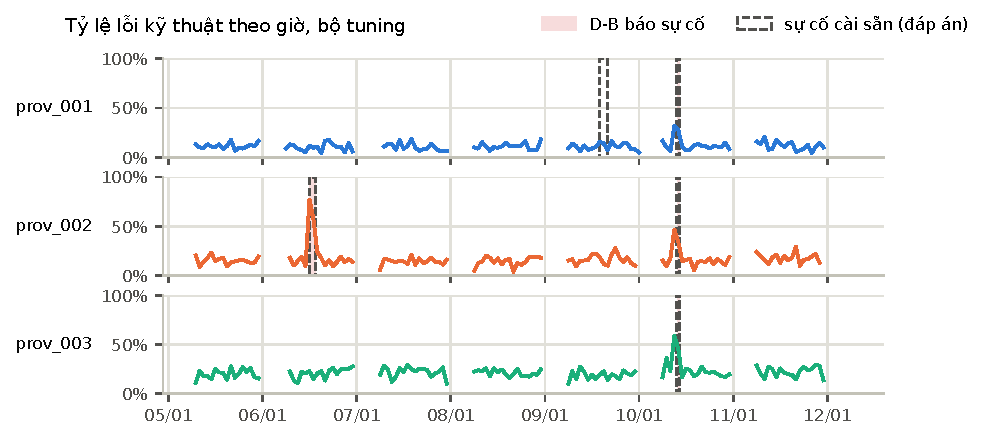
\includegraphics[width=0.92\textwidth]{figures/p01_failure.pdf}

  {\scriptsize\color{ink2} Mỗi provider một hàng, cùng thang. Vùng đỏ: D-B báo sự cố; khung nét đứt:
  sự cố cài sẵn (đáp án, người vận hành thật không có). Ẩn giờ có dưới 20 attempt.}
\end{frame}

% ---------------------------------------------------------------------
\begin{frame}{Hai detector}
  \begin{columns}[T]
    \begin{column}{0.48\textwidth}
      \begin{block}{D-A: z-score bền vững (đường cơ sở)}\small
        So mỗi khung 15 phút với trung vị và MAD của cùng khung giờ những ngày trước.
        \begin{itemize}\small
          \item đơn giản, dễ giải thích
          \item nhạy với khung ít attempt $\Rightarrow$ báo nhầm
        \end{itemize}
      \end{block}
    \end{column}
    \begin{column}{0.48\textwidth}
      \begin{block}{D-B: nhị thức gộp cửa sổ (chính)}\small
        Gộp số lỗi / số attempt trong một cửa sổ, kiểm định nhị thức so với đường nền 24 giờ.
        \begin{itemize}\small
          \item tính đúng cỡ mẫu nhỏ
          \item ngưỡng chỉnh trên bộ tuning, rồi khoá
        \end{itemize}
      \end{block}
    \end{column}
  \end{columns}
  \vspace{4mm}
  \begin{alertblock}{Quy trình chống “chỉnh theo đáp án”}\small
    Ngưỡng chỉnh trên bộ \textbf{tuning}; bộ \textbf{report} (seed khác, có một loại sự cố chưa gặp)
    đánh giá \textbf{một lần} bằng \texttt{make detect-report}, ghi sổ \texttt{detect\_report\_runs.json}.
  \end{alertblock}
\end{frame}

% ---------------------------------------------------------------------
\begin{frame}{Kết quả Product 01}
  \begin{columns}[c]
    \begin{column}{0.5\textwidth}
      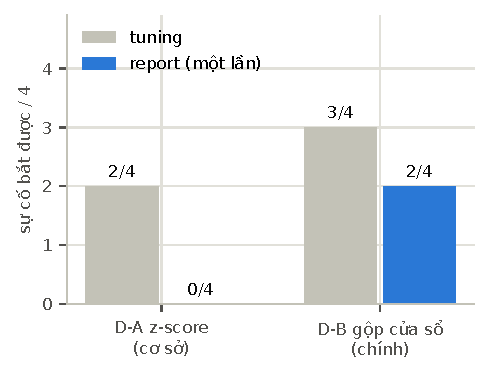
\includegraphics[width=\textwidth]{figures/p01_detectors.pdf}
    \end{column}
    \begin{column}{0.48\textwidth}\small
      \begin{tabular}{@{}lcc@{}}
        \toprule
        & Tuning & Report\quoted \\
        \midrule
        D-B (chính) & \num{3/4} · 0,0 & \num{2/4} · 0,0 \\
        D-A (cơ sở) & 2/4 · 1,0 & 0/4 · 2,0 \\
        \bottomrule
      \end{tabular}\\[1mm]
      {\scriptsize sự cố bắt được · báo nhầm/ngày}

      \vspace{3mm}
      \begin{itemize}\small
        \item D-B: không báo nhầm ở cả hai bộ; bắt trong 15–30 phút
        \item Sự cố x1,5 nằm dưới giới hạn phát hiện
        \item Report thấp hơn tuning: đúng như kỳ vọng khi khoá ngưỡng trước
      \end{itemize}
      \src{det-3ddc26cff253 · det-08335c6af086}
    \end{column}
  \end{columns}
\end{frame}

% =====================================================================
\section{Product 02 · Fraud \& Risk}

\begin{frame}{Pipeline Product 02}
  \centering
  \begin{tikzpicture}[node distance=3mm]
    \node[pstep] (a) {\faFileCsv\\IEEE-CIS\\\num{590.540}\\giao dịch};
    \node[pstep,right=of a] (b) {\faFingerprint\\Manifest\\checksum\\SHA-256};
    \node[pstep,right=of b] (c) {\faCut\\Chia thời gian\\60 / 20 / 20};
    \node[pstep,right=of c] (d) {\faProjectDiagram\\Đặc trưng\\fit trên train};
    \node[pstep,right=of d] (e) {\faBrain\\Luật · LR\\· GBM};
    \node[pstep,right=of e] (f) {\faSlidersH\\Hiệu chỉnh\\(V1) · chính\\sách (V2)};
    \node[pstep,right=of f] (g) {\faLayerGroup\\Chấm điểm\\theo lô};
    \foreach \x/\y in {a/b,b/c,c/d,d/e,e/f,f/g} \draw[arr] (\x)--(\y);
    \node[pstep,draw=bad,below=6mm of e,text width=30mm] (t) {\faLock\ Tập test: \textbf{một lần}\\PR-AUC 0,408\quoted};
    \draw[arr,dashed,bad] (e) -- (t);
  \end{tikzpicture}

  \vspace{1mm}
  \begin{columns}[T]
    \begin{column}{0.48\textwidth}
      \begin{block}{Chống rò rỉ}\footnotesize
        Nhãn tách khỏi đặc trưng; đặc trưng chỉ dùng quá khứ; mọi tiền xử lý fit trên train;
        ngưỡng chọn trên validation.
      \end{block}
    \end{column}
    \begin{column}{0.48\textwidth}
      \begin{block}{Không dùng accuracy}\footnotesize
        Gian lận chỉ $\approx$3,5\%: báo “không gian lận” cho mọi giao dịch đã đúng 96,5\%.
        Dùng \textbf{PR-AUC} (kèm CI bootstrap), recall tại FPR cố định.
      \end{block}
    \end{column}
  \end{columns}
\end{frame}

% ---------------------------------------------------------------------
\begin{frame}{Chất lượng xếp hạng: ba mô hình}
  \begin{columns}[c]
    \begin{column}{0.52\textwidth}
      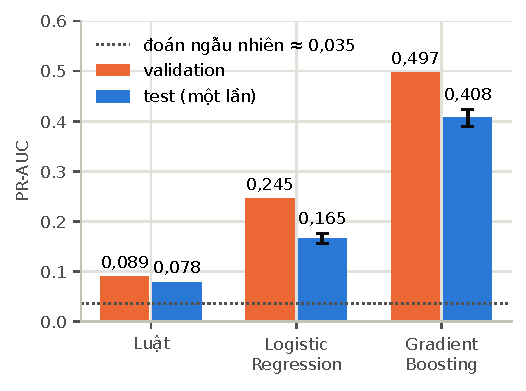
\includegraphics[width=\textwidth]{figures/p02_prauc.pdf}
    \end{column}
    \begin{column}{0.46\textwidth}\small
      \begin{tabular}{@{}lccc@{}}
        \toprule
        Mô hình & Valid & Test\quoted & R@FPR5\% \\
        \midrule
        Luật & 0,089 & 0,078 & 0,22 \\
        Logistic & 0,245 & 0,165 & 0,28 \\
        \textbf{GBM} & \textbf{0,497} & \textbf{0,408} & \textbf{0,51} \\
        \bottomrule
      \end{tabular}\\[1mm]
      {\scriptsize GBM test 95\% CI [0,390; 0,424]}

      \vspace{1mm}
      \begin{itemize}\footnotesize
        \item GBM gấp $\approx$12 lần mức đoán ngẫu nhiên
        \item Valid > test: validation đã bị dùng để chọn
        \item Recall@FPR5\% chọn ngưỡng bằng nhãn của chính tập test: đo \emph{thứ tự}, không phải hiệu quả triển khai
      \end{itemize}
      \src{run-d6faa4699008 · run-f8807cb6f780}
    \end{column}
  \end{columns}
\end{frame}

% ---------------------------------------------------------------------
\begin{frame}{Ngưỡng đã chốt trước khi mở test, và thí nghiệm rò rỉ}
  \begin{columns}[T]
    \begin{column}{0.48\textwidth}
      \begin{block}{GBM, ngưỡng 0,853 (chọn trên validation)}
        \centering\small
        \begin{tabular}{@{}lr@{}}
          Precision (test) & \num{0,516}\\
          Recall (test) & \num{0,371}\\
          FPR (test) & \num{1,24\%}\\
        \end{tabular}
      \end{block}
      \vspace{2mm}
      {\scriptsize\color{ink2} Điểm vận hành FPR 1,24\% khác điểm FPR 5\% ở slide trước: không đọc là
      recall “tụt từ 51\% xuống 37\%”.}
    \end{column}
    \begin{column}{0.48\textwidth}
      \begin{alertblock}{Thí nghiệm rò rỉ (validation)}
        \footnotesize
        Mã hoá \texttt{card1} bằng nhãn: PR-AUC \textbf{+0,063}\\
        Chia ngẫu nhiên thay vì theo thời gian: \textbf{−0,068}\\[2mm]
        Rò nhãn làm điểm \emph{đẹp giả}. Chia ngẫu nhiên lại cho điểm \emph{thấp hơn}:
        phần lớn chênh lệch do hai tập validation không cùng dòng.
      \end{alertblock}
      \src{leak-827d929eaa73}
    \end{column}
  \end{columns}
\end{frame}

% =====================================================================
\section{Stage G · Từ điểm số đến quyết định (thăm dò)}

\begin{frame}{Điểm có đọc được như xác suất không? Hiệu chỉnh}
  \centering
  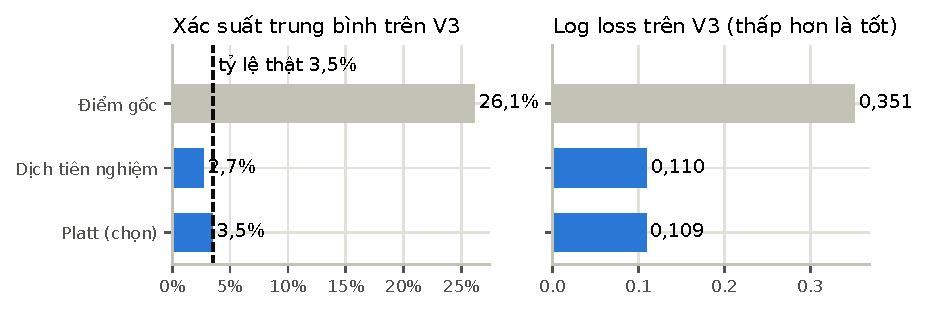
\includegraphics[width=0.88\textwidth]{figures/p02_calibration.pdf}

  \vspace{2mm}
  \begin{columns}[T]
    \begin{column}{0.9\textwidth}\small
      \begin{itemize}
        \item Điểm gốc trung bình \num{26,1\%}, gian lận thật \num{3,5\%}: \textbf{thổi lên $\approx$7 lần}
              (do \texttt{class\_weight="balanced"}).
        \item Platt fit trên V1, chọn trên V2, đo trên V3: log loss \num{0,351 → 0,109}.
        \item Hiệu chỉnh đơn điệu \textbf{không đổi PR-AUC}; nó chỉ quan trọng khi đặt ngưỡng theo chi phí.
      \end{itemize}
    \end{column}
  \end{columns}
  \src{cal-04b3ad5944ce} {\scriptsize\color{ink2}· chỉ train + validation}
\end{frame}

% ---------------------------------------------------------------------
\begin{frame}{So sánh chính sách quyết định (chi phí giả định)}
  \begin{columns}[c]
    \begin{column}{0.6\textwidth}
      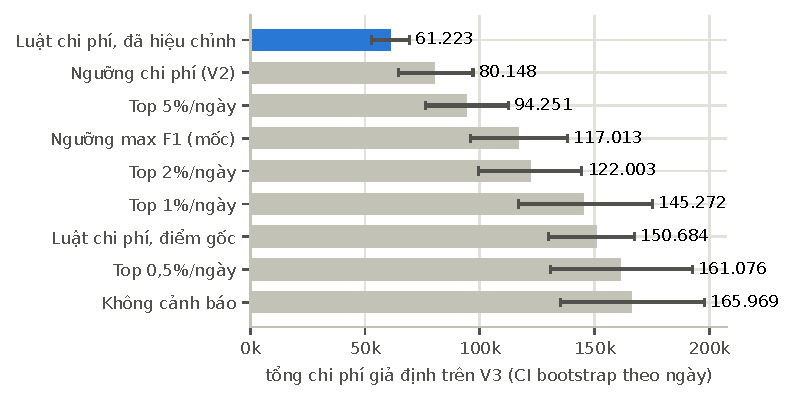
\includegraphics[width=\textwidth]{figures/p02_policy.pdf}
    \end{column}
    \begin{column}{0.38\textwidth}\footnotesize
      Chi phí giả định (đơn vị tương đối):
      \begin{itemize}\footnotesize
        \item bỏ sót: $0{,}75 \times$ số tiền
        \item mỗi lần duyệt: 5
        \item mỗi cảnh báo nhầm: 1
      \end{itemize}
      \vspace{2mm}
      Luật chi phí dùng xác suất \textbf{đã hiệu chỉnh} rẻ nhất ở \num{27/27} tổ hợp chi phí.

      \vspace{2mm}
      {\scriptsize\color{bad}\textbf{Phân tích độ nhạy, không phải ROI.} Một phần do luật được
      chấm bằng chính hàm chi phí nó tối ưu.}
    \end{column}
  \end{columns}
  \src{pol-af5df43efe54 · V3 · L0.75/R5/F1}
\end{frame}

% ---------------------------------------------------------------------
\begin{frame}{Ngưỡng chọn hôm nay có giữ được ngày mai? Độ ổn định}
  \begin{columns}[T]
    \begin{column}{0.44\textwidth}
      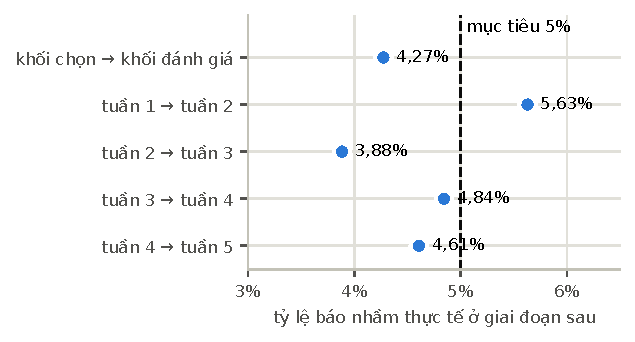
\includegraphics[width=\textwidth]{figures/p02_transfer.pdf}
      {\scriptsize Ngưỡng FPR 5\% chọn ở khối trước cho FPR thực tế \num{3,9–5,6\%} ở khối sau.}
    \end{column}
    \begin{column}{0.55\textwidth}
      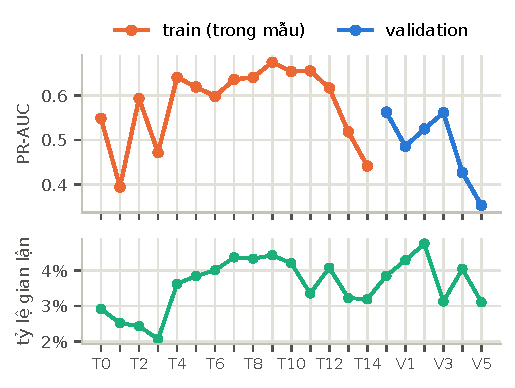
\includegraphics[width=\textwidth]{figures/p02_stability.pdf}
      {\scriptsize PR-AUC tuần validation \num{0,35–0,56}. PSI 4 đầu vào < 0,05: trôi phân phối
      \emph{không} giải thích được hai tuần cuối.}
    \end{column}
  \end{columns}
  \src{pol-af5df43efe54 · stab-36887d48b356}
\end{frame}

% ---------------------------------------------------------------------
\begin{frame}{Chấm điểm theo lô (G08)}
  \begin{columns}[c]
    \begin{column}{0.5\textwidth}
      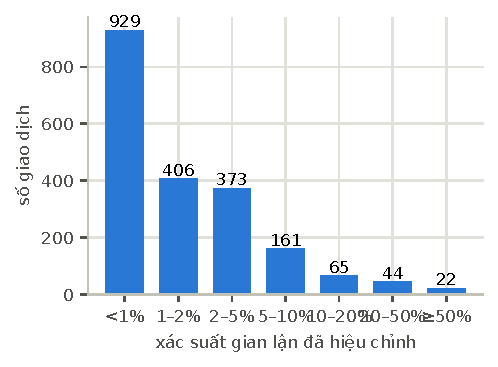
\includegraphics[width=\textwidth]{figures/p02_scores.pdf}
    \end{column}
    \begin{column}{0.48\textwidth}\footnotesize
      \texttt{make score-model} rồi \texttt{make score}
      \begin{itemize}\footnotesize
        \item \num{2.000} giao dịch V3 \textbf{không nhãn}
        \item lệch huấn luyện–chấm điểm: \num{0} (cùng dòng, cùng điểm)
        \item ghi \texttt{model\_version}, \texttt{feature\_version}, \texttt{execution\_id}
        \item \textbf{từ chối} file có cột nhãn hoặc dòng thuộc giai đoạn test
      \end{itemize}
      \vspace{2mm}
      Phá hoại có chủ đích: lệch \texttt{hour\_of\_day} 7 giờ lúc chấm $\Rightarrow$ 2 test báo lỗi.
      \\[2mm]\src{score-19e94be9616d}
    \end{column}
  \end{columns}
\end{frame}

% =====================================================================
\section{Kỹ thuật, chất lượng và demo}

\begin{frame}{Dashboard: một trang, mở offline}
  \centering
  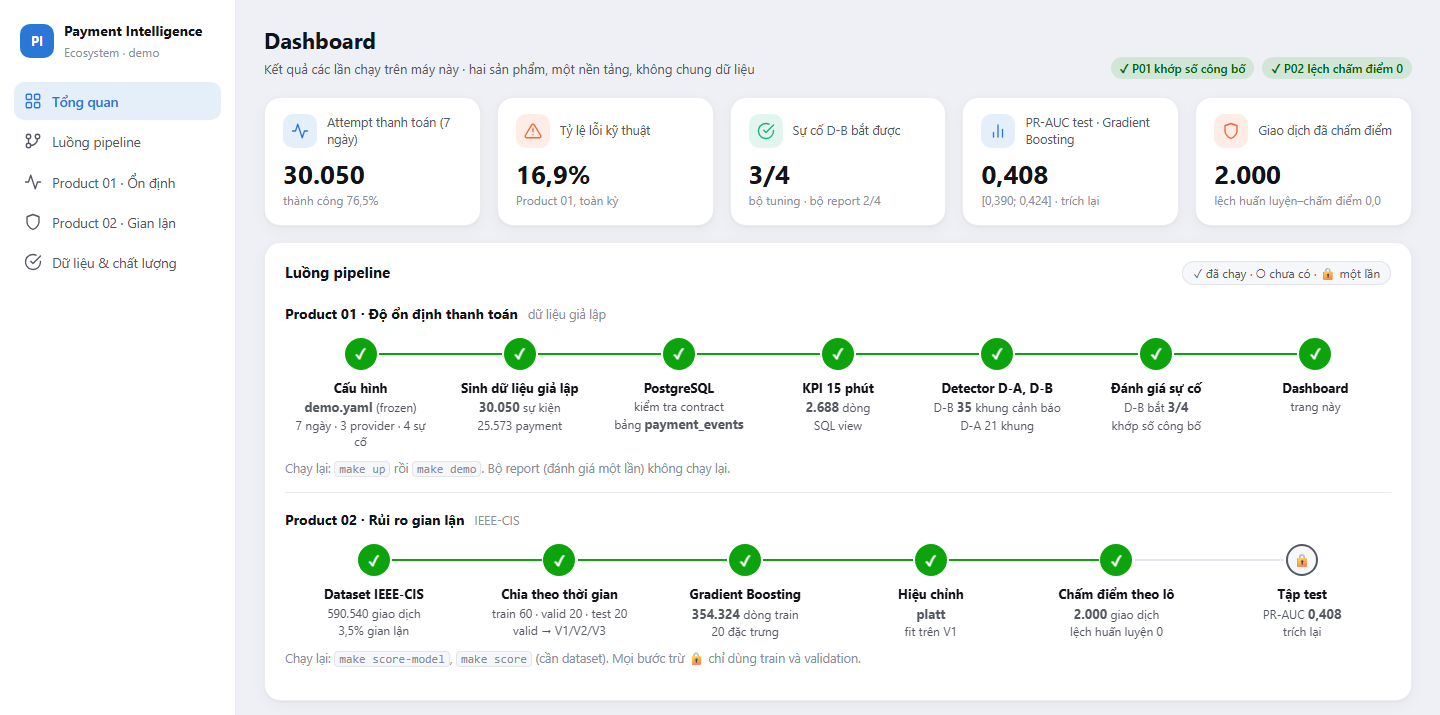
\includegraphics[width=0.86\textwidth]{figures/dashboard_top.png}

  {\scriptsize\color{ink2} \texttt{make demo} → \texttt{artifacts/dashboard/index.html}: số liệu chính,
  luồng pipeline, biểu đồ có tooltip, sáng/tối.\\ Số test chỉ trích từ \texttt{results/published.json}.}
\end{frame}

% ---------------------------------------------------------------------
\begin{frame}{Chất lượng phần mềm}
  \begin{columns}[c]
    \begin{column}{0.5\textwidth}
      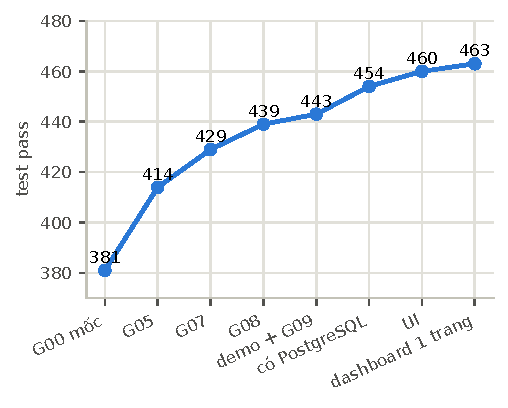
\includegraphics[width=\textwidth]{figures/tests_progress.pdf}
    \end{column}
    \begin{column}{0.48\textwidth}\small
      \begin{itemize}\small
        \item \num{463} test pass, 1 skip (có PostgreSQL thật)
        \item CI: lint + test trên Python 3.11 và 3.13, PostgreSQL 16, job \texttt{make demo},
              job kiểm sổ test-một-lần
        \item \num{11} ADR cho mọi quyết định kiến trúc
        \item Tự kiểm tra mỗi task: đảo nhãn, nhìn tương lai, tính lại độc lập, phá hoại có chủ đích,
              chạy hai lần trùng từng byte
      \end{itemize}
    \end{column}
  \end{columns}
\end{frame}

% ---------------------------------------------------------------------
\begin{frame}{Demo trong 5 phút}
  \begin{columns}[T]
    \begin{column}{0.5\textwidth}
      \begin{tabular}{@{}l@{\quad}l@{}}
        \texttt{make setup} & môi trường + git hook\\
        \texttt{make up} & PostgreSQL 16 (Docker)\\
        \texttt{make demo} & cả hai sản phẩm\\
      \end{tabular}\\[3mm]
      \small
      Terminal (thư viện \texttt{rich}, ADR 0011): sản phẩm đang chạy, \% tiến độ,
      bảng kết quả, danh sách kiểm tra \textcolor{good}{\faCheck} / \textcolor{bad}{\faTimes}.
    \end{column}
    \begin{column}{0.46\textwidth}
      \begin{exampleblock}{Kiểm tra tự động khi demo}\small
        \faCheck\ D-B 3/4, 0 báo nhầm/ngày (khớp công bố)\\
        \faCheck\ D-A 2/4, 1,0 báo nhầm/ngày\\
        \faCheck\ lệch chấm điểm = 0\\
        \faCheck\ không đụng bộ report, không đọc test
      \end{exampleblock}
      \small Product 02 cần dataset IEEE-CIS trong \texttt{datasets/raw/} (không commit).
    \end{column}
  \end{columns}
\end{frame}

% =====================================================================
\section{Hạn chế và hướng tiếp theo}

\begin{frame}{Hạn chế: kết quả này \emph{không} chứng minh}
  \begin{itemize}
    \item Product 01 dùng dữ liệu \textbf{giả lập}, mỗi bộ chỉ \textbf{4 sự cố}: kiểm chứng trên bất thường
          đã biết, không phải tỷ lệ phát hiện thực tế.
    \item Product 02: \texttt{C1–C14} mang gần hết tín hiệu (bỏ chúng: PR-AUC validation 0,497 → 0,158),
          ý nghĩa chưa xác minh.
    \item Validation đã dùng nhiều lần (lưới GBM, rò rỉ, Stage G): số trên validation có thể \textbf{lạc quan}.
    \item Chi phí Stage G là \textbf{giả định}: phân tích độ nhạy, không phải ROI.
    \item Giả định nhãn gian lận có ngay; thực tế chargeback đến muộn nhiều tuần.
    \item Hai sản phẩm chưa chung dữ liệu; không API, không giám sát mô hình, không huấn luyện lại.
  \end{itemize}
\end{frame}

% ---------------------------------------------------------------------
\begin{frame}{Hướng tiếp theo}
  \begin{columns}[T]
    \begin{column}{0.48\textwidth}
      \begin{block}{Ngắn hạn}\small
        \begin{itemize}
          \item Merge chuỗi PR Stage G vào \texttt{main}, xác nhận CI xanh
          \item G10 (chờ duyệt): sự cố \emph{tăng dần} để thử D-B có bị “luộc ếch”;
                nạp trùng / muộn / hỏng, tải 10×; lật nhãn x\% trên train
        \end{itemize}
      \end{block}
    \end{column}
    \begin{column}{0.48\textwidth}
      \begin{block}{Dài hạn (ngoài phạm vi demo)}\small
        \begin{itemize}
          \item Nối hai sản phẩm qua \texttt{payment\_id} từ cùng nguồn sự kiện
          \item Mở rộng sang hệ thống con khác (đối soát, chargeback)
          \item API chấm điểm, giám sát trôi mô hình
        \end{itemize}
      \end{block}
    \end{column}
  \end{columns}
\end{frame}

% ---------------------------------------------------------------------
\begin{frame}[standout]
  Cảm ơn đã lắng nghe!\\[4mm]
  {\normalsize Hỏi đáp}\\[2mm]
  {\footnotesize\texttt{github.com/TrungTuyenDo02/Payment\_Intelligence\_Ecosystem}}
\end{frame}

\end{document}
